\section{Outlier detection}


\subsection{Outliergrams}

\textcite{gil-romo-2014} combined the notions of the modified epigraph index
(MEI) and the modified band depth (MBD), proposing the outliergram as a tool
for detecting shape outliers.
They show that for a sample $\{\vx_i\}_{i = 1}^n$, each
\begin{equation}
    \MBD(\vx_i) = D_{MB}(\vx_i, \hat{F}_n) \leq a_0 + a_1 \MEI(\vx_i) + a_2 n^2 \MEI(\vx_i)^2
\end{equation}
where $a_0 = a_2 = -2/n(n - 1)$ and $a_1 = 2(n + 1)/(n - 1)$.
The distance
\begin{equation}
    d_i = a_0 + a_1 \MEI(\vx_i) + a_2 n^2 \MEI(\vx_i) - \MBD(\vx_i)
\end{equation}
is indicative of the outlyingness of $\vx_i$.
\textcite{gil-romo-2014} consider shape outlying curves as those for which
$d_i \geq d^* = Q_3 + 1.5\IQR$, where $Q_3$ and $\IQR$ are the third quartile
and the interquartile range of $\{d_i\}_{i = 1}^n$ respectively.
The graph $\{(\MEI(\vx_i), \MBD(\vx_i))\}_{i = 1}^n$ is called the
\emph{outliergram}.
Shape outliers are those whose $(\MEI, \MBD)$ falls outside a ribbon of height
$d^*$ under the parabola $a_0 + a_1 x^2 + a_2n^2x^2$.

\begin{figure}
    \centering
    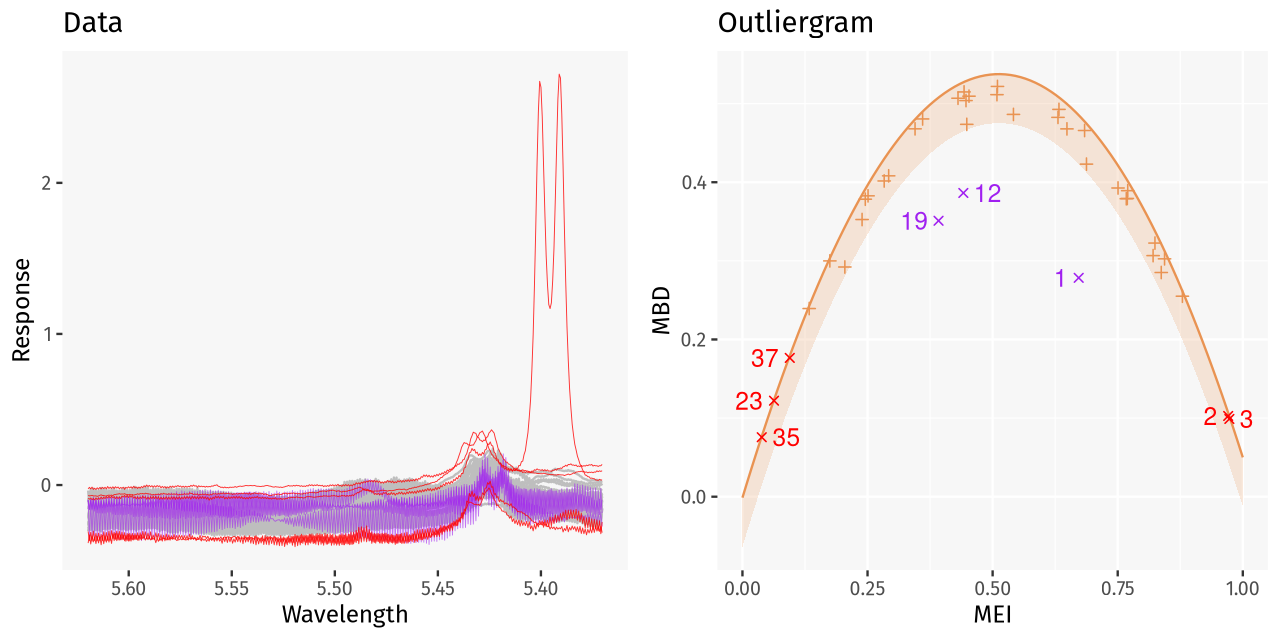
\includegraphics[width = \textwidth]{outliergram_wine}
    \caption{
        Outliergram for the NMR spectra of 40 wine samples.
        The three purple curves have been identified as shape outliers, as
        they fall outside the orange ribbon in the outliergram.
        Although the red curves lie on the orange parabola, they have low MBD
        and extreme MEI values, indicating that they lie above or below the
        main mass of curves.
    }
    \label{fig:outliergram_wine}
\end{figure}



\subsection{Centrality-stability diagrams}

In their discussion of methods of functional outlier detection,
\textcite{hubert-rousseeuw-segeart-2015} proposed the centrality-stability
diagram, where both the `centrality' of a curve (measured by depth) and its
variability in cross-sectional outlyingness over time are accounted for.

We observe that the MO-VO diagram from \textcite{dai-genton-2018} neatly falls
under a general category of centrality-stability diagrams.


\begin{figure}
    \centering
    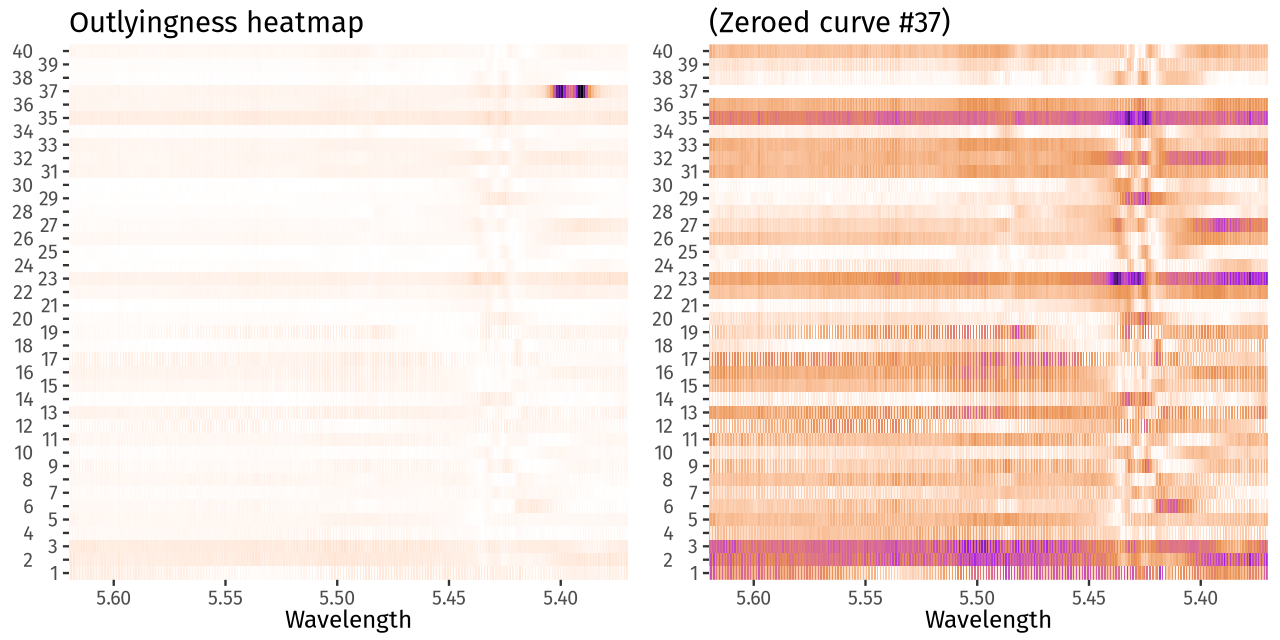
\includegraphics[width = \textwidth]{outlyingness_heatmap_wine}
    \caption{
        Outlyingness heatmap for the NMR spectra of 40 wine samples.
        The extreme curve \#37 has been zeroed out in the second diagram to
        better illustrate the variation in outlyingness for the remaining
        curves.
    }
    \label{fig:outlyingness_heatmap_wine}
\end{figure}

\begin{figure}
    \centering
    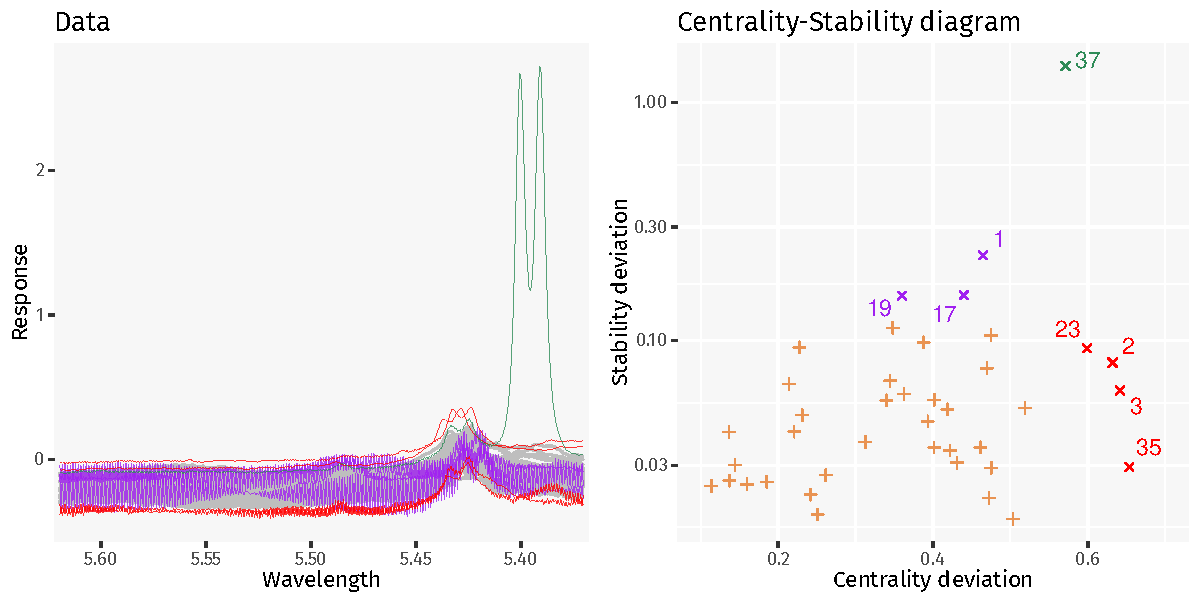
\includegraphics[width = \textwidth]{centrality_stability_wine}
    \caption{
        Centrality-stability diagram for the NMR spectra of 40 wine samples.
        The red curves are seen to deviate in terms of centrality, indicated
        by the fact that the corresponding points in the centrality-stability
        diagram fall towards the right.
        The purple curves deviate in terms of stability, with the green curve
        showing extreme deviation.
    }
    \label{fig:centrality_stability_wine}
\end{figure}

\begin{figure}
    \centering
    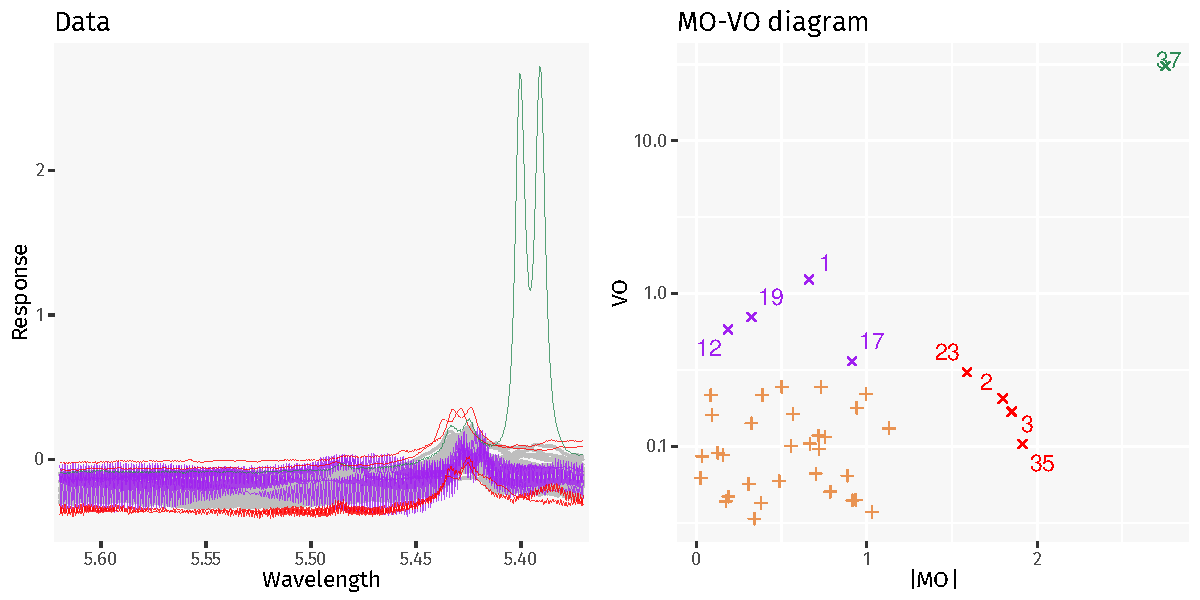
\includegraphics[width = \textwidth]{MO_VO_wine}
    \caption{
        MO-VO diagram for the NMR spectra of 40 wine samples.
    }
    \label{fig:MO_VO_wine}
\end{figure}





\begin{figure}
    \centering
    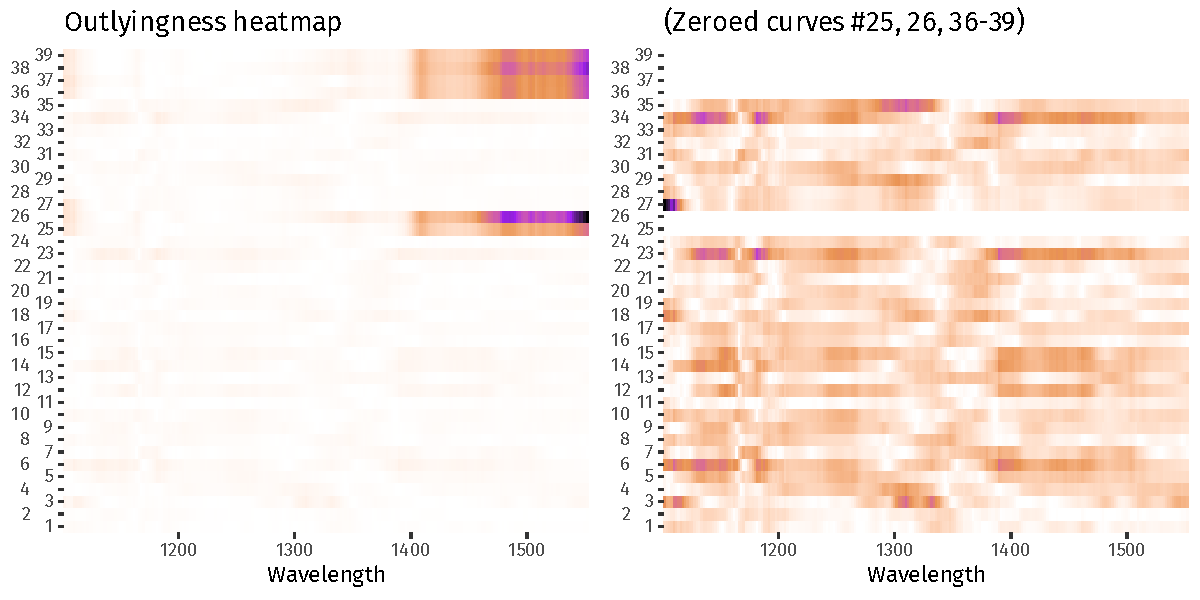
\includegraphics[width = \textwidth]{outlyingness_heatmap_octane}
    \caption{
        Outlyingness heatmap for the NIR spectra of 39 gasoline samples.
        The outlying curves have been zeroed out in the second diagram.
    }
    \label{fig:outlyingness_heatmap_octane}
\end{figure}

\begin{figure}
    \centering
    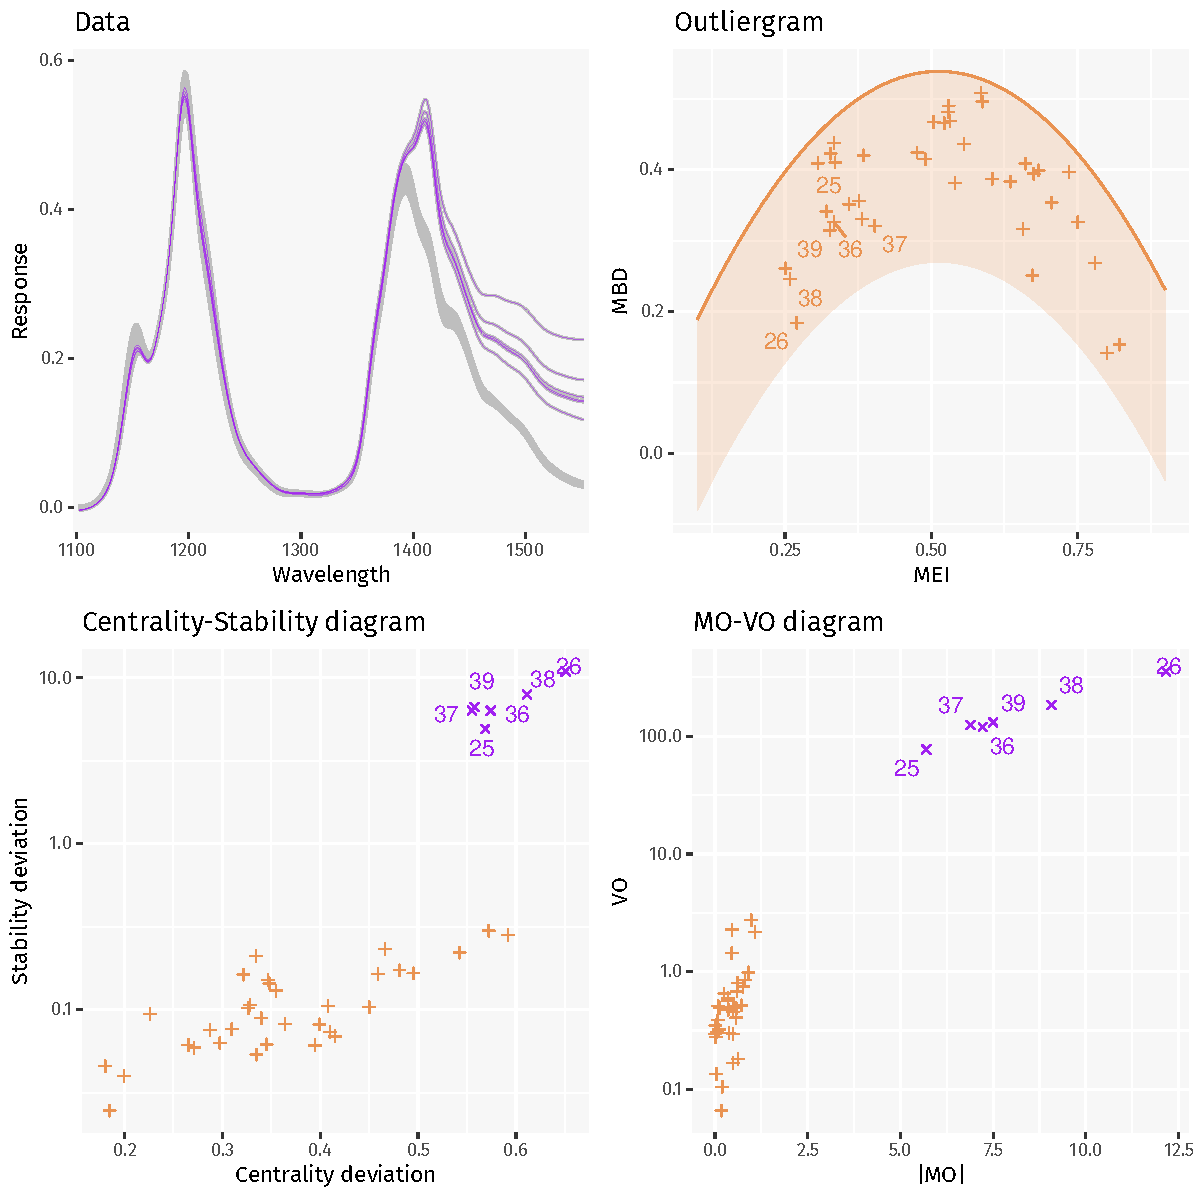
\includegraphics[width = \textwidth]{outlyingness_octane}
    \caption{
        Outliergram, centrality-stability, and MO-VO diagrams for the NIR
        spectra of 39 gasoline samples.
        The six purple curves \#25, 26, 36-39 correspond to samples containing
        added alcohol.
        While the outliergram does not clearly identify these outliers, the
        centrality-stability and MO-VO diagrams show a marked separation from
        the main curves.
    }
    \label{fig:outlyingness_octane}
\end{figure}



